% KSe.tex
% $Author$ $Date$

% Predrag                   jun 20 2006
% Vaggelis                  may 20 2006

\section{\KSe}
\label{s-KS}
% Predrag                    4jul2006
% extracted from ~dasbuch/book/chapter/PDEs.tex  5jun2005 version
% Predrag                   17sep1999

% \PC{incorporate missing refs from chapter/refsPDEs.tex}

The \KS\ [KS] system\rf{ku,siv}, which
arises in the description of stability of
flame fronts, reaction-diffusion systems and many other physical settings,
is one of the simplest nonlinear PDEs that
exhibit spatiotemporally chaotic behaviour.
In the formulation adopted here, the time evolution of the 
``flame front velocity'' $u=u(x,t)$ defined on a periodic domain
$u(x,t) = u(x+L,t)$
is given by
\beq
    u_t=(u^2)_x-u_{xx}- u_{xxxx}
    \,,\qquad   x \in [0,2\pi \tildeL]
    \,.
\ee{ks}
Here $t \geq 0$ is the time and
$x$ is the spatial coordinate.
The subscripts $x$ and $t$ denote partial derivatives with respect to
$x$ and $t$. We shall use interchangeably the ``dimensionless''
system size $\tildeL$, or the periodic domain size $L= 2\pi \tildeL$,
as the single system parameter.

Spatial periodic boundary condition $u(x,t)=u(x+L,t)$
makes it convenient to work in the Fourier space, 
\beq
  u(x,t)=\sum_{k=-\infty}^{+\infty} a_k (t) e^{ i k x /\tildeL }
\, .
% \label{fseries}
\ee{eq:ksexp}
where $\tildeL=L/2\pi$. Thus, \refeq{ks} is replaced by an infinite set of 
ODEs for the Fourier coefficients:
\beq
\dot{a}_k= \left( k/\tildeL \right)^2.
      \left( 1 - \left( k/\tildeL \right)^2  \right) a_k 
    + i \frac{k}{\tildeL} \sum_{m=-\infty}^{+\infty} a_m a_{k-m}
\,.
\ee{expan}
Since $u(x,t)$ is real,
$ %\[
a_k=a_{-k}^*
\,,
$ %\] %\label{cplx-b}
so we can replace the sum over $k$ in \refeq{expan} by a
sum over $k \geq 0$.
As  $\dot{a_0}=0$, $a_0$ is a conserved quantity,
in our calculations
fixed to $a_0=0$ by
the Galilean invariance condition \refeq{GalInv}.



\subsection{Symmetries of \KSe}
% former \subsection{Scaling and symmetries}
% former symm.tex
% Predrag extracted from newton.tex         jul  3 2006

The  KS equation is
Galilean invariant: if $u(x,t)$ is a solution, then 
$v+u(x+2vt,t)$, with $v$ an arbitrary constant velocity, is also a solution. 
Without loss of generality, in our calculations we shall set 
the mean velocity of the  front to zero,
% \index{Galilean invariance}
% \index{invariance!Galilean}
\beq
\int dx \, u = 0
\,.
\ee{GalInv}
The KS equation  \refeq{ks} is time translationally invariant,
and 
space translationally invariant
under the 1-$d$ Lie group of $O(1)$ rotations: if
$u(x,t)$ is a solution, then $u(x+d,t)$ is an equivalent
solution for any $-L/2 < d \leq L/2$.
As a result,
KS can have \rpo\ solutions with nonzero shift
\beq
u(x+d,\period{}) = u(x,0)
\,.
\ee{KSrpos}
where $\period{}$ is the period.
\ES{Is this obvious to everybody? I cannot really see why it is so.}
The KS equation is also invariant under
reflection (``parity'' or ``inversion'') operation
\beq
\Refl u(x) = -u(-x)
\ee{KSparity}
and the shift symmetry operation 
\beq
\Shift u(x)=u(x+L/2)
\,. 
\ee{KSshift}
In the Fourier modes decomposition  this
symmetry corresponds to invariance under
\refeq{FModInvSymm}.
This shift symmetry is a particular case of the
above translational $O(2)$ invariance; more generally,
KS allows for solutions invariant under any rational shift by
$L/m$. Any \rpo\ with such rational shift is eventually periodic.
\Rpo s without a discrete symmetry have irrational shifts
$d$, and are not segments of a periodic solution.


Relations $\Refl^2=\Shift^2=1$
induce a linear decomposition of the space of solutions into 4 invariant
subspaces\rf{KNSks90} via projection operators
$\Refl_1=(\matId+\Refl)/2$,
$\Refl_2=(\matId-\Refl)/2$,
$\Shift_1=(\matId+\Shift)/2$, and
$\Shift_2=(\matId-\Shift)/2$. The nonlinear term $(u^2)_x$ in the KS equation
mixes these subspaces, leading,
according to \refref{KNSks90}, to four invariant subspaces
(labeled by the corresponding projection operators):
\begin{itemize}
 \item[$R_1$:] The space of antisymmetric functions,
 \item[$S_1$:] The space of L/2 periodic functions,
 \item[$R_1 S_1$:] The intersection of the above two,
 \item[$L$:] The space of functions invariant under $x\mapsto L/2-x,\ u\mapsto -u$.
 
\end{itemize}
%\ES{Using notation of \rf{KNSks90} here, not sure if it exists elsewere.}
The dynamics within the $R_1$ space of antisymmetric functions
was studied in \refref{Christiansen:97,Lan:Thesis,lanCvit06}.

\subsection{Bifurcation structure of \KS}
\label{sec:KSlit}
% former KSlit.tex
%
% Vaggelis               jan 20 2007
% \subsection{\Eqva\ according to Greene and Kim}

In our study of the \eqva\ of
\KSe\ we follow the bifurcations analysis of
Kevrekidis, Nicolaenko and Scovel\rf{KNSks90} 
and
Greene and Kim\rf{ksgreene88}. What is new here is
a detailed exploration of the \eqva\ stable/unstable manifolds
for a specific system size $L = 22$, determination
of a large number of \rpo s, and a preliminary
exploration of the relation between the
observed spatiotemporal ``turbulent" patterns and
the \rpo s computed so far.


% What is the non-dimensional ``Rayleigh'' number for the
% \KS\ system? 
%  Scaling out the ``viscosity'' $\nu$ 
% \[ 
% x \to x \nu^{\frac{1}{2}}
% \,,\quad
% t \to t \nu
% \,,\quad
% u \to u \nu^{-\frac{1}{2}}
% \,,
% \]
% brings the \KSe\ \refeq{ks}
% to a non-dimensional form
% \beq
% u_t=(u^2)_x-u_{xx}- u_{xxxx}
% \,,\qquad 
%   x \in  [0,L\nu^{-\frac{1}{2}}] = [0,2\pi\tilde{L}]
% \,.
% \ee{ks-L}
% In this way the ``viscosity'' $\nu$
% and the system size $L$ are trade in for a single
% dimensionless system size parameter
% \beq
%   \tilde{L}={L}/{(2 \pi \sqrt{\nu})}
% % \tilde{L}=\frac{L}{2 \pi \sqrt{\nu}}
% % \,,
% \ee{tildeL}
% which plays the role of a ``Reynolds number''
% for the \KS\ system.

In the literature \refeq{ks} is sometimes written as
\beq
    u_t=(u^2)_x-u_{xx}- \nu \, u_{xxxx}
    \,,\qquad   x \in [0,L]
    \,,
\ee{ksVisc}
or in any number of other variants, all equivalent.
We use
$L$ as the system parameter, with the ``hyperviscosity" $\nu$ fixed to $1$, 
At other times $\nu$ is varied with $L$ fixed to either $1$ or $2\pi$.
To minimize confusion,
in what follows we shall state results of all 
calculations either in units of the dimensionless system size $\tildeL$,
or the systems size $L = 2 \pi \tildeL$. The parameter $\alpha$
of \refrefs{KNSks90,ksgreene88} in this convention is
$\tildeL=\sqrt{\alpha/4}$.


For small $\tildeL$ the only \eqv\ of the system is the constant solution $y(x,t)=0$,
globally attracting 
for $\tildeL<1$. At $\tildeL=N$, $N=1,2,3, \dots$, 
the $N$th harmonic becomes unstable and the constant solution
bifurcates to the antisymmetric ``$N$-cell'' states\rf{ksgreene88}. 
These states contain only the multiples of the $N$th
harmonic, {\ie}, only the components $a_N,a_{2N},...$ in our notation.
Greene and Kim show that symmetric solutions are \eqva, not \reqva. 
% At point $A$ in \reffig{fig:GreeneKim}
At point $A$ in \reffig{fig:ksBifDiag}
the $1$-cell state loses stability
and bifurcates to a stable, 
asymmetric \reqv, which later on becomes unstable through a Hopf bifurcation. 

At $\tildeL=2$ the system has become large enough 
that a $2$-cell \eqv\ appears. 
% At point $B$ in \reffig{fig:GreeneKim}
At point $B$ in \reffig{fig:ksBifDiag}
the $1$-cell branch merges to the $2$-cell branch. 
In general each $N$-cell branch merges to the corresponding $2N$-cell branch.

% At point $C$ in \reffig{fig:GreeneKim}
At point $C$ in \reffig{fig:ksBifDiag}
the $2$-cell state bifurcates to a type of 
\eqv\ solution
found by La Quey, Mahajan, Rutherford and Tang\rf{laquey74} and generalized by Greene and Kim who refer to them as GLMRT \eqva. GLMRT solutions are symmetric 
($u(x)$ is antisymmetric)
and can be roughly described as long-wave distorted $N$-cell states.

% The last type of solution identified in \refref{ksgreene88} appears at point $F$ 
% in \reffig{fig:GreeneKim} and is called a
% ``giant" state because its amplitude grows as the system size increases.

According to the bifurcation diagram 
% \reffig{fig:GreeneKim}, 
\reffig{fig:ksBifDiag}, 
at the point that corresponds to system size $\tildeL=22/2\pi \simeq 3.5$
studied here,
the {\eqva} we expect are the $2$- and $3$-cell states $\EQV{2}$ and $\EQV{3}$,
the GLMRT state that bifurcates from a $3$-cell state at point $I$ ($\EQV{1}$),
the pair of \reqva\ that belong to the branches starting at points $A$ ($\REQV{\pm}{1}$),
and the $M$ branch  \reqva\ $\REQV(\pm){2}$.


% In \reffig{fig:GreeneKim} 
In \reffig{fig:ksBifDiag} 
the ``elastic energy'' reads:
\beq
    \tilde{E}=\frac{1}{L}\int_0^{L}\tilde{u}^2\, d\tilde{x}
    \,.
\label{ksEnergy}
\eeq


%%%%%%%%%%%%%%%%%%%%%%%%%%%%%%%%%%%%%%%%%%%%%%%%%%%%%%%%%%%%%%%%
% \begin{figure}[t]
%     % \vspace*{-5pt}
% \centering
% 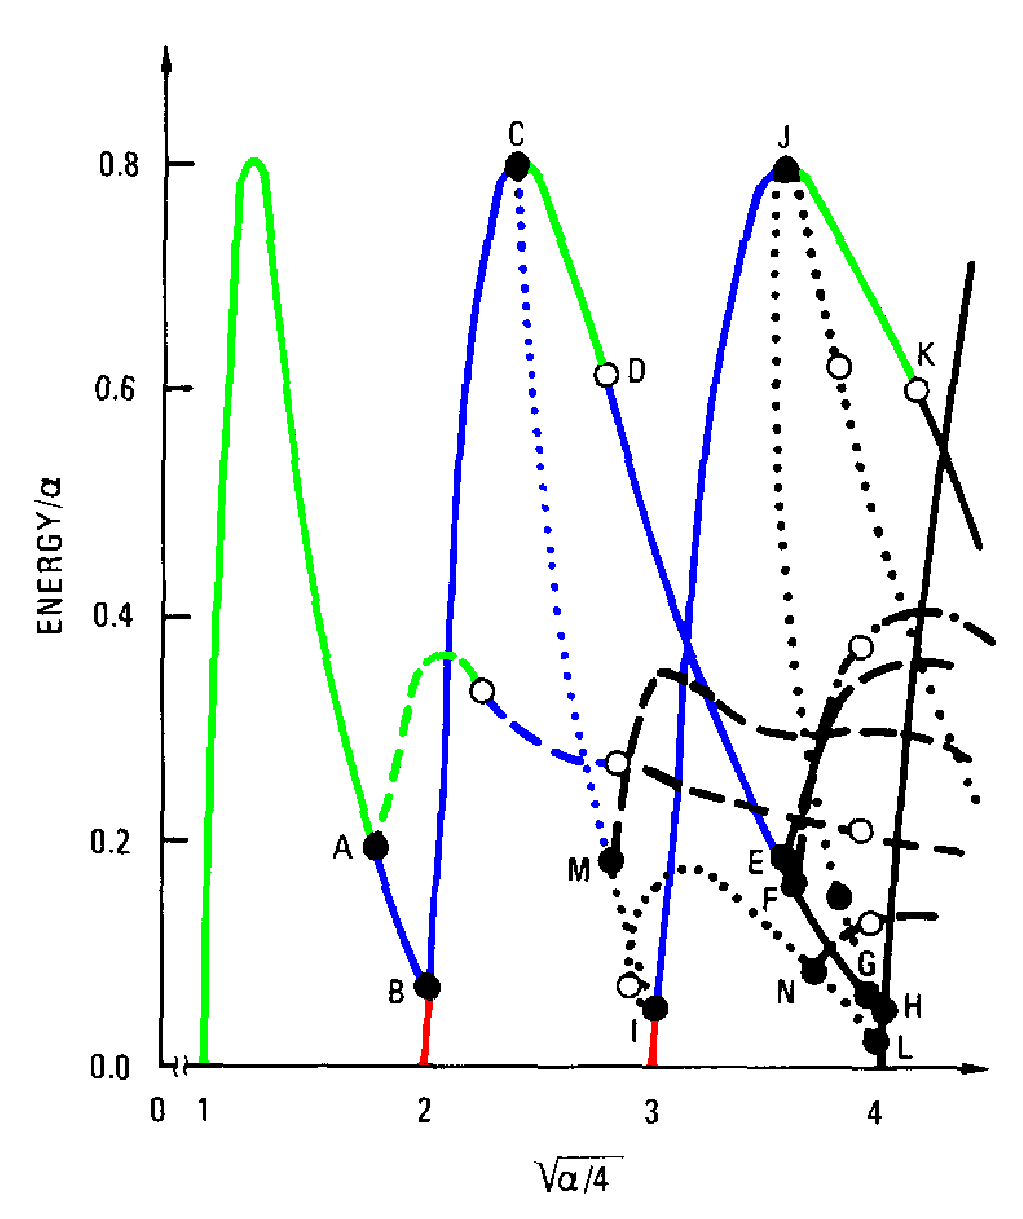
\includegraphics[width=0.5\textwidth]{figs/GreeneKimBifColor.eps}
%     % \vspace*{-5pt}
% \caption{
%     {\small
% The ``energy'' of \eqva\ as a function of the bifurcation
% parameter $\tildeL=\sqrt{\alpha}/2$, from \refref{ksgreene88}.
% The solid curves denote $N$-cell solutions,
% dotted curves GLMRT, the dash-dotted curve the
% giant states, and dashed curves the propagating solutions.
% Open circles indicate Hopf bifurcations. 
% We have color-coded the branches to reflect the number of unstable
% eigenvalues (or complex pairs). Red: 2 unstable eigenvalues, Blue: 1
% unstable eigenvalue, Green: stable. Solutions not 
% resolved in \refref{ksgreene88} or of no interest
% to our present purposes have been left black.
%         } %end \small
%         }
% \label{fig:GreeneKim}
%     % \vspace*{-5pt}
% \end{figure}
%%%%%%%%%%%%%%%%%%%%%%%%%%%%%%%%%%%%%%%%%%%%%%%%%%%%%%%%%%%%%%%%%%


%%%%%%%%%%%%%%%%%%%%%%%%%%%%%%%%%%%%%%%%%%%%%%%%%%%%%%%%%%%%%%%%
\begin{figure}[t]
{\centering
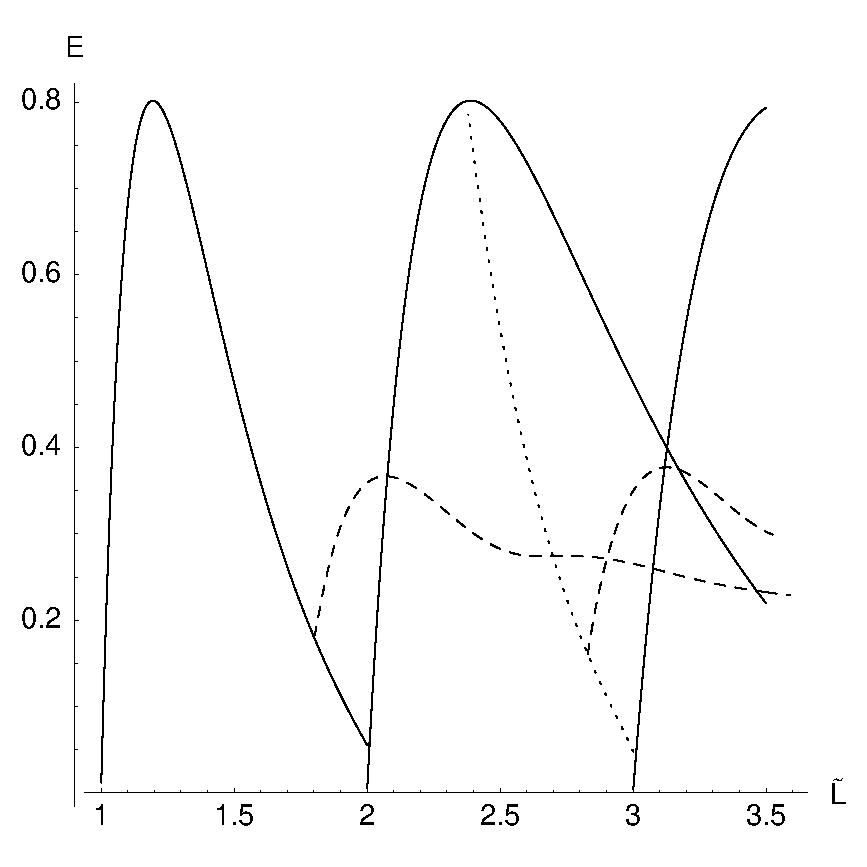
\includegraphics[width=0.5\textwidth]{figs/ksBifDiag.eps}
}
\caption{
    {\small
The ``energy'' \refeq{ksEnergy}  of \eqva\
plotted as a function of the system size
$\tildeL$ (recomputed following \refref{ksgreene88}), tracked to
$\tildeL \approx 3.5$ studied here.
Solid curves denote $N$-cell solutions,
dotted curves GLMRT, the dash-dotted curve the
giant states, and dashed curves the propagating solutions.
Open circles indicate Hopf bifurcations. 
The color of a branch indicates the number of unstable
eigenvalues: (red) 2 unstable eigenvalues, (blue) 1
unstable eigenvalue, (green) stable. 
\ESedit{
ES: Shown is the 2c to GLMRT bifurcation and the GLMRT to $\REQV{\pm}{2}$ bifurcation, 
points C and M in \rf{ksgreene88} respectively.
       } 
    } %end \small
        }
\label{fig:ksBifDiag}
\end{figure}
%%%%%%%%%%%%%%%%%%%%%%%%%%%%%%%%%%%%%%%%%%%%%%%%%%%%%%%%%%%%%%%%%%

        \PublicPrivate{%
        }{% switch to Private:

\subsection{Back in the saddle again}

Kevrekidis, Nicolaenko and Scovel~\rf{KNSks90} study \KSe\ steady state 
bifurcations and the role of symmetry in the existance of structurally stable (relative) homoclinic and heteroclinic connections between unstable saddles. The form  of the equation they use is
essentially that of Greene and Kim but with bifurcation parameter connected to our by $\alpha=4\tilde{L}^2$.


They prove that the bifurcation of the trivial state $y=0$ to an $N$-cell state is a pitchfork. 
They observe that when the $1$-cell state losses stability at point $A$ the
eigenvector corresponding to the zero eigenvalue of the stability matrix aligns itself with the direction of uniform translation of the
system which, due to the translational invariance of \KSe\, also corresponds to a zero eigenvalue. Thus the algebraic multiplicity of the zero eigenvalue is $2$ while its geometric multiplicity is $1$. Using this fact and a local, $O(2)$-equivariant, approximation to the center manifold they prove that this type of bifurcation creates traveling waves.

In typical numerical simulations  a trajectory initiated along the (single) unstable eigendirection of a
fixed point $y$ of the $2$-cell branch would eventually become attracted to the $L/4$-translated equilibrium $y'$. 
Those (relative) homoclinic connections 
\ES{In \refref{KNSks90} the characterization homoclinic connection is used. Here
we prefer (to invent?) the term relative homoclinic to emphasize the fact that the fixed points are symmetry related.} although structurally unstable in most dynamical systems, were found to be persistent in KSe with the afore-mentioned behaviour observed in the range  
from $\tilde{L}\simeq 2.009$ up to $\tilde{L}\simeq 2.375$  where the $2$-cell state becomes stable. The existance and
robustness of the saddle connection was explained as follows\ES{The following may not make perfect sense without reading the paper, especially the
notation. I've start re-writing \KS\ symmetries section to incorporate information about the invariant subspaces which hopefully will explain it but
my progress is very slow.}:  The unstable manifold of $y$ lies on an invariant subspace $L$ of
\KS\ flow, which is the fixed set of the isotropy subgroup of $O(2)$ defined by reflection with respect to imaginary axis. The action of the generator of $D(4)$ (which sents y to y') on $L$ is to send it to the invariant subspace $R_{1}$ which is the fixed set of $Z(2)$ defined by complex
conjugation. The converse is also true, i.e. the action of $D(4)$ sents $R_{1}$ to $L$. Thus the unstable eigendirection of $y$, lying on $L$, is sent on $R_{1}$ for the $L/4$-shifted point $y'$. The two invariant subspaces $L$ and $R_{1}$ are orthogonal and thus the point $y'$ has only stable eigendirections on $L$ and appears as a sink on that subspace. This explains why the (relative) homoclinic connections are structurally stable in \KSe.

In the range $\tilde{L}=2.00$ when the $2$-cell branch comes to existance with two unstable eigendirections, up to $\tilde{L} \simeq 2.009$ when it
merges to the $1$-cell branch and losses one of its unstable eigendirections, a heteroclinic loop exists that connects $2$-cell to $1$-cell solutions.
The analysis is similar to the previous case.

An important remark in \refref{KNSks90} is that the exact saddle connections were observed using a numerical integrator based on an explicit Galerkin spectral discretezation of \KSe, irrespective of how close to the equilibrium along the unstable manifold we start. On the contrary, when an FFT-based integrator was used, trajectories with initial condition along the unstable direction of $y$ would approach the homoclinic connection but fly away along the direction of the unstable manifold of $y'$ and follow an approximate (relative) homoclinic loop. This is attributed to the Galerkin truncation respecting the symmetries and possesing the same subspaces as the original equation restricted to the first $n$ modes \ES{We observe the second kind of behavour and we both use an FFT based integrator. I plan to quikly write a Galerkin integrator and check to see if we get an exact connection.}.

        } %end \PublicPrivate{%

